\documentclass{standalone}
\usepackage[utf8]{inputenc}
\usepackage{pgfplots}
\DeclareUnicodeCharacter{2212}{−}
\usepgfplotslibrary{groupplots,dateplot}
\usetikzlibrary{patterns,shapes.arrows}
\pgfplotsset{compat=newest}
\begin{document}
% This file was created by tikzplotlib v0.9.4.
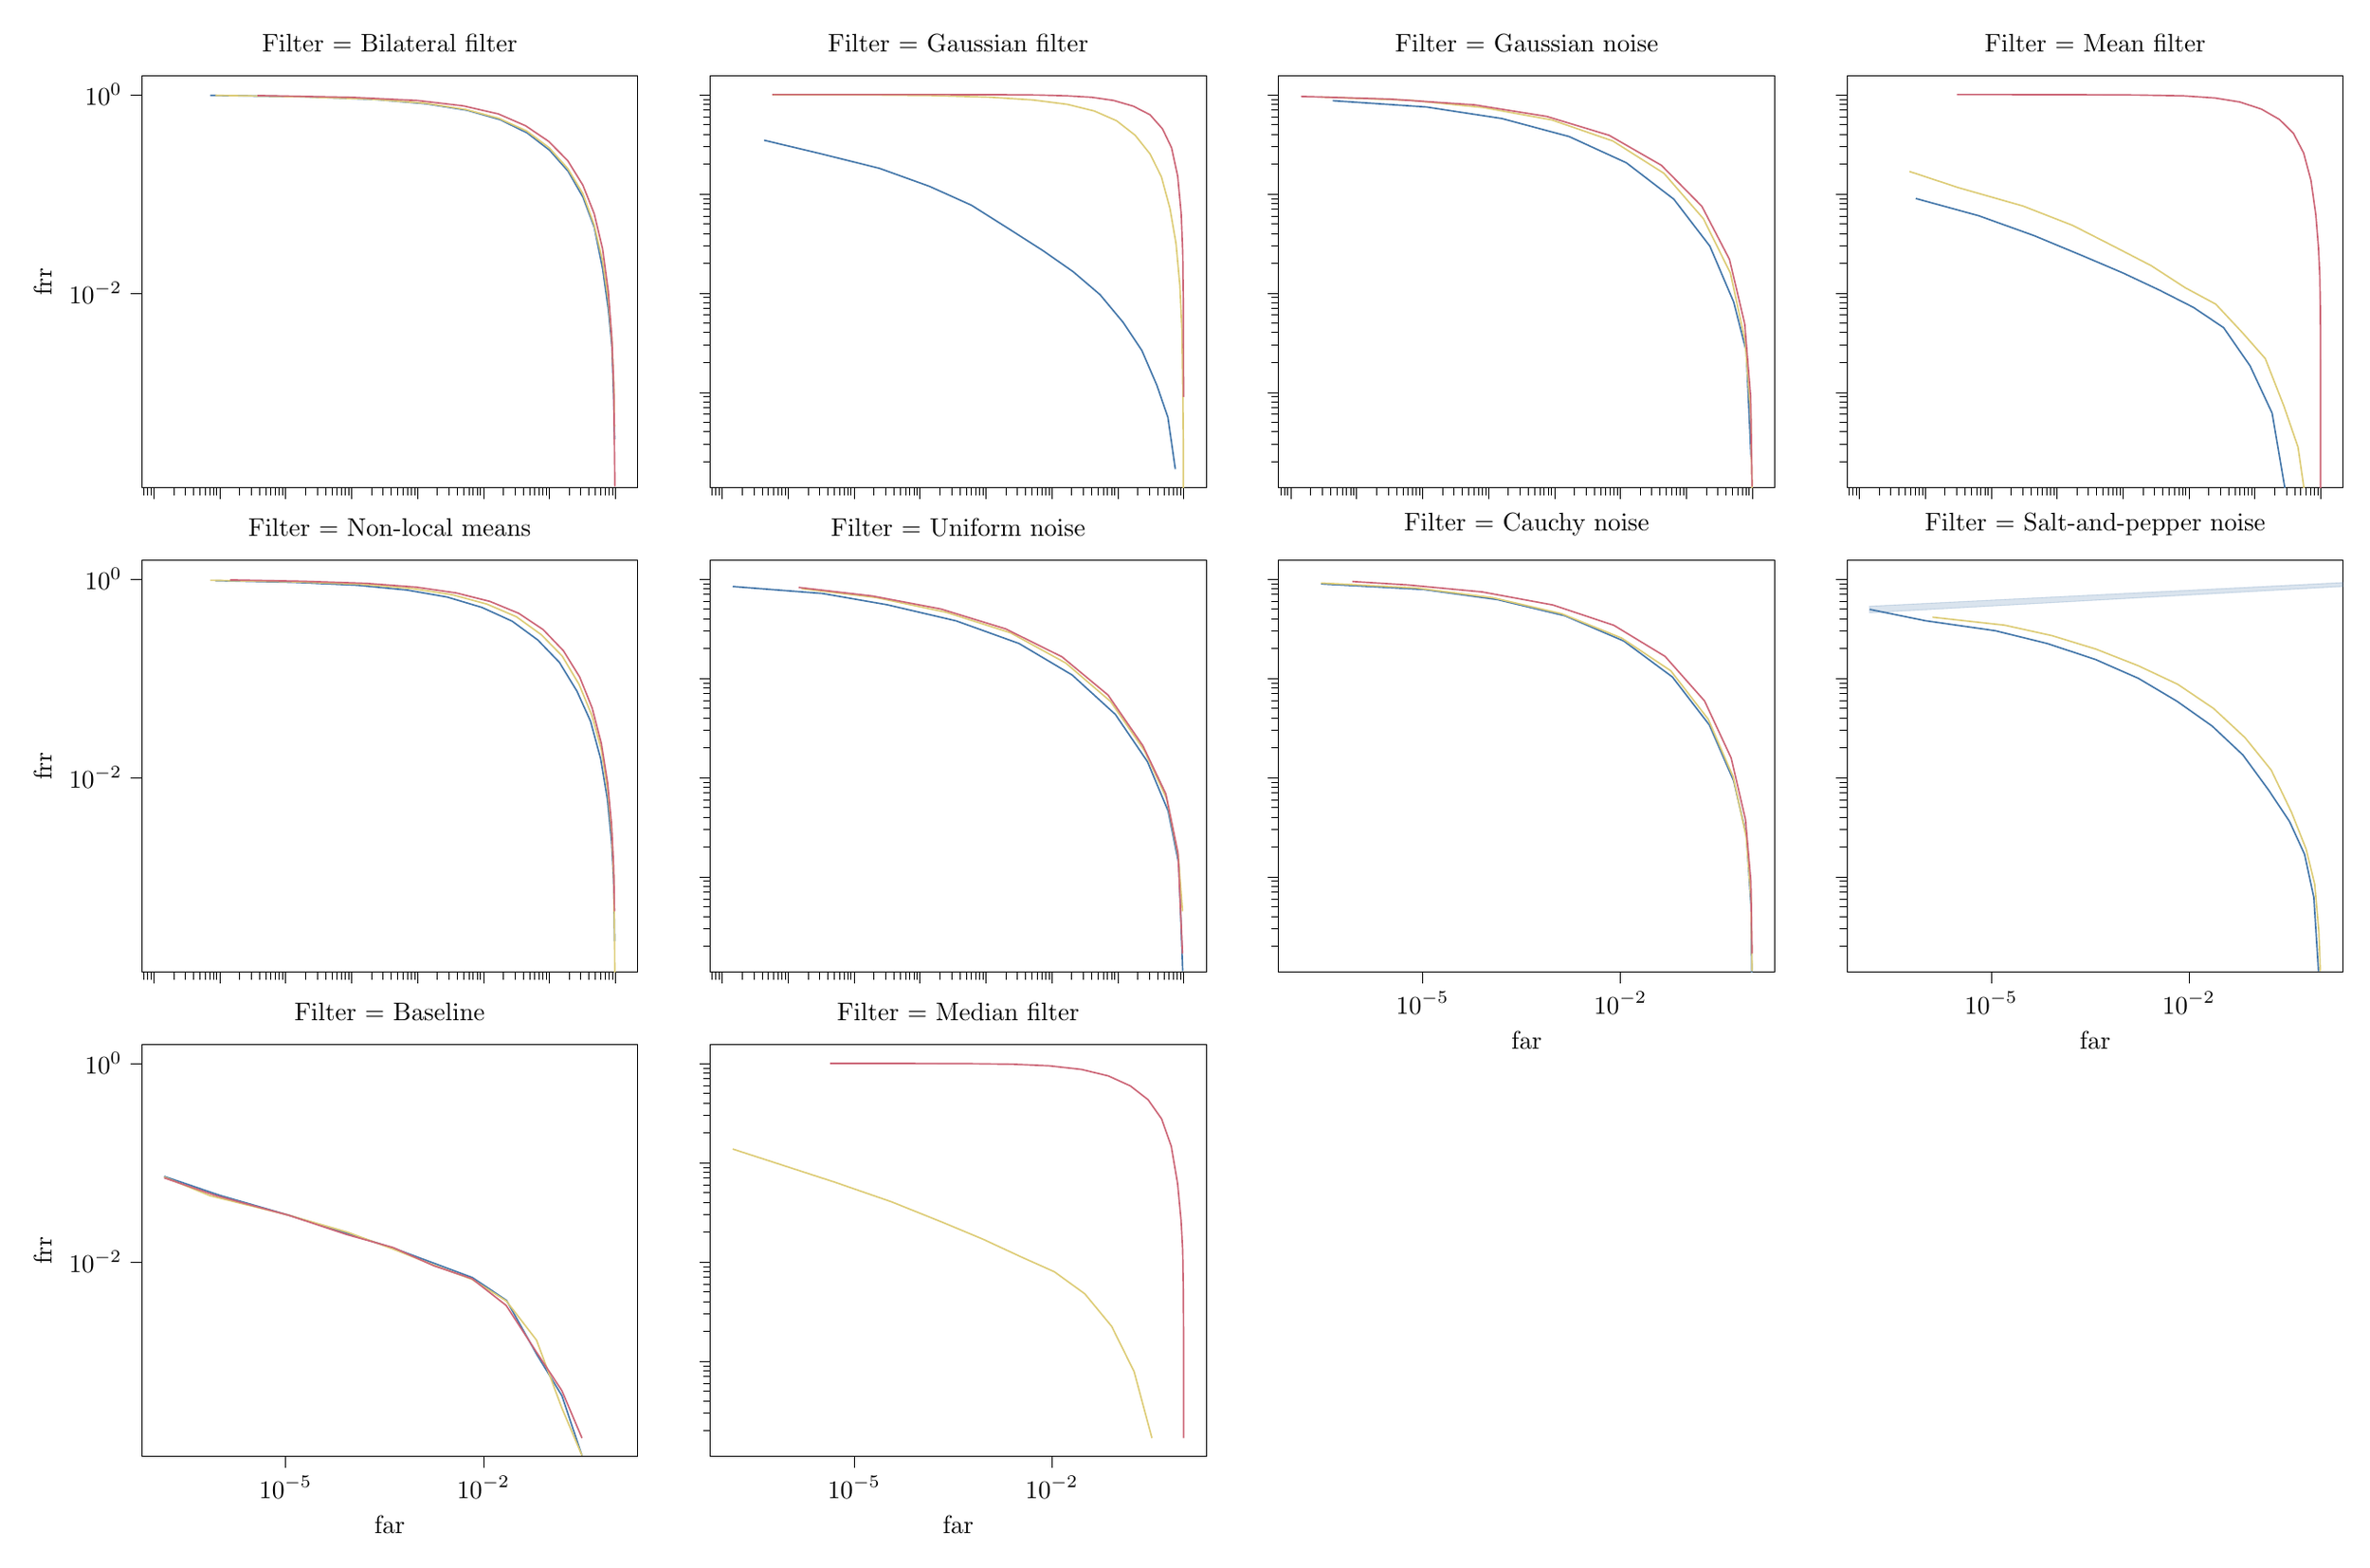
\begin{tikzpicture}

\definecolor{color0}{rgb}{0.266666666666667,0.466666666666667,0.666666666666667}
\definecolor{color1}{rgb}{0.866666666666667,0.8,0.466666666666667}
\definecolor{color2}{rgb}{0.8,0.4,0.466666666666667}

\begin{groupplot}[group style={group size=4 by 3}]
\nextgroupplot[
log basis x={10},
log basis y={10},
scaled x ticks=manual:{}{\pgfmathparse{#1}},
tick align=outside,
tick pos=left,
title={Filter = Bilateral filter},
x grid style={white!69.0196078431373!black},
xmin=6.55121351783882e-08, xmax=2.19826434799841,
xmode=log,
xtick style={color=black},
xticklabels={},
y grid style={white!69.0196078431373!black},
ylabel={frr},
ymin=0.00010874258979921, ymax=1.54433983109274,
ymode=log,
ytick style={color=black},
ytick={1e-06,0.0001,0.01,1,100,10000},
yticklabels={\(\displaystyle {10^{-6}}\),\(\displaystyle {10^{-4}}\),\(\displaystyle {10^{-2}}\),\(\displaystyle {10^{0}}\),\(\displaystyle {10^{2}}\),\(\displaystyle {10^{4}}\)}
]
\path [draw=color0, fill=color0, opacity=0.2]
(axis cs:0,0.999998000767705)
--(axis cs:0,0.99916572036338)
--(axis cs:0,0.999998000767705)
--(axis cs:0,0.999998000767705)
--cycle;
\path [draw=color0, fill=color0, opacity=0.2]
(axis cs:1,0)
--(axis cs:1,0)
--(axis cs:1,0)
--(axis cs:1,0)
--cycle;

\path [draw=color1, fill=color1, opacity=0.2]
(axis cs:0,1)
--(axis cs:0,0.99934360205681)
--(axis cs:0,1)
--(axis cs:0,1)
--cycle;
\path [draw=color1, fill=color1, opacity=0.2]
(axis cs:1,0)
--(axis cs:1,0)
--(axis cs:1,0)
--(axis cs:1,0)
--cycle;

\path [draw=color2, fill=color2, opacity=0.2]
(axis cs:0,1)
--(axis cs:0,0.999171421622373)
--(axis cs:0,1)
--(axis cs:0,1)
--cycle;
\path [draw=color2, fill=color2, opacity=0.2]
(axis cs:1,0)
--(axis cs:1,0)
--(axis cs:1,0)
--(axis cs:1,0)
--cycle;

\addplot [semithick, color0]
table {%
0 0.999702114388075
7.20064955619517e-07 0.98191894312584
2.03058317484704e-05 0.950291088222123
0.000234885188523086 0.892465293327362
0.00134580140205288 0.808385579937304
0.00558828010757194 0.696092700403045
0.0179592840710975 0.558217644424541
0.0461277930959596 0.410714285714286
0.101370168400151 0.274238692342141
0.193248872594299 0.168607254814151
0.324381197779089 0.0923645320197044
0.48216211888042 0.045846394984326
0.645403436553205 0.0174652933273623
0.787862815528863 0.00677339901477833
0.889978683197054 0.00291088222122705
0.949685317213095 0.000839677563815495
0.977557015463251 0.000335871025526198
0.989093176117231 0
0.995059778352486 0
0.998596593401498 0
0.999811486994619 0
0.999990063103612 0
1 0
};
\addplot [semithick, color1]
table {%
0 0.999748096730855
8.6407794674342e-07 0.982982534706673
1.52653770591338e-05 0.95230631437528
0.000198161875786491 0.90013434841021
0.00127926740015363 0.820085087326467
0.0054133043233564 0.708128078817734
0.017367102651596 0.574339453649798
0.0452125905373672 0.429802955665025
0.0998404624084329 0.29064039408867
0.19124363570589 0.179019256605464
0.321561999464848 0.100873264666368
0.478475242294657 0.0489811912225705
0.64119105656283 0.0214397671294223
0.784250105633529 0.00867666815942678
0.887466952618862 0.00341468875951635
0.948238706717256 0.00123152709359606
0.976828741767137 0.000447828034034931
0.988764106432513 0
0.994882642373403 0
0.998455316657205 0
0.999759354291832 0
0.999982718441065 0
0.999999279935044 0
1 0
};
\addplot [semithick, color2]
table {%
0 0.999685362200226
3.74433776922149e-06 0.977888490819525
0.000103545340618086 0.937360053739364
0.00100981909376081 0.870633676668159
0.0049765129212776 0.768752798925213
0.0168305102466683 0.638434841021048
0.0437740447690305 0.484381997313032
0.0977555863359322 0.337606359158083
0.190800507732202 0.215405284370802
0.32322160517456 0.122201074787282
0.481142074864289 0.0627519032691446
0.643913334134046 0.0278213166144201
0.786376601460465 0.0104120017913121
0.888429247425552 0.00352664576802508
0.948546030440314 0.00117554858934169
0.977038712708196 0.000223914017017465
0.988601803791516 0.000111957008508733
0.994364771657322 0
0.998199261558987 0
0.999754313837143 0
0.999988046921737 0
0.999999855987009 0
1 0
};

\nextgroupplot[
log basis x={10},
log basis y={10},
scaled x ticks=manual:{}{\pgfmathparse{#1}},
scaled y ticks=manual:{}{\pgfmathparse{#1}},
tick align=outside,
tick pos=left,
title={Filter = Gaussian filter},
x grid style={white!69.0196078431373!black},
xmin=6.55121351783882e-08, xmax=2.19826434799841,
xmode=log,
xtick style={color=black},
xticklabels={},
y grid style={white!69.0196078431373!black},
ymin=0.00010874258979921, ymax=1.54433983109274,
ymode=log,
ytick style={color=black},
yticklabels={}
]
\path [draw=color0, fill=color0, opacity=0.2]
(axis cs:0,0.976713591980679)
--(axis cs:0,0.877670724441814)
--(axis cs:0,0.976713591980679)
--(axis cs:0,0.976713591980679)
--cycle;
\path [draw=color0, fill=color0, opacity=0.2]
(axis cs:1,0)
--(axis cs:1,0)
--(axis cs:1,0)
--(axis cs:1,0)
--cycle;

\path [draw=color1, fill=color1, opacity=0.2]
(axis cs:0,1)
--(axis cs:0,0.999988004606231)
--(axis cs:0,1)
--(axis cs:0,1)
--cycle;
\path [draw=color1, fill=color1, opacity=0.2]
(axis cs:1,0)
--(axis cs:1,0)
--(axis cs:1,0)
--(axis cs:1,0)
--cycle;

\path [draw=color2, fill=color2, opacity=0.2]
(axis cs:0,1)
--(axis cs:0,1)
--(axis cs:0,1)
--(axis cs:0,1)
--cycle;
\path [draw=color2, fill=color2, opacity=0.2]
(axis cs:1,0)
--(axis cs:1,0)
--(axis cs:1,0)
--(axis cs:1,0)
--cycle;

\addplot [semithick, color0]
table {%
0 0.929577042415712
4.3203897337171e-07 0.34628302731751
3.02427281360197e-06 0.254646215853112
2.41941825088158e-05 0.180586654724586
0.000139692601390186 0.118730407523511
0.000602982393835783 0.0766905508284819
0.00220095054334661 0.0445588893864756
0.00729022563667423 0.0268137035378415
0.0211772543577611 0.016345723242275
0.0538042615748281 0.00962830273175101
0.119676379766866 0.00509404388714734
0.232471818817832 0.00263098969995522
0.391651970140922 0.00117554858934169
0.575580753988656 0.000559785042543663
0.747260080837372 0.000167935512763099
0.873940820453531 0
0.946993426383007 0
0.980924759260683 0
0.994341585565751 0
0.998772865302633 0
0.999834241047216 0
0.999990207116604 0
1 0
};
\addplot [semithick, color1]
table {%
0 0.99999600153541
5.76051964495613e-07 0.998768472906404
8.928805449682e-06 0.994793999104344
0.000146317198981886 0.97833631885356
0.00113395829210961 0.941894312583968
0.00517913919978893 0.882165248544559
0.0171431624503983 0.796742051052396
0.0440717196216836 0.683105687416032
0.0961880049275485 0.543831168831169
0.183509418017581 0.388994626063592
0.307912880205098 0.25268696820421
0.459130697261939 0.148343036274071
0.619566497854638 0.0709807433945365
0.765606039789637 0.0315158978952082
0.874666501915805 0.0119793999104344
0.94090470113128 0.00425436632333184
0.973380206681684 0.000951634572324228
0.986926788691754 0.000335871025526198
0.993563915413682 5.59785042543663e-05
0.997724882766225 0
0.999555143870418 0
0.999953483803867 0
0.999997839805133 0
1 0
};
\addplot [semithick, color2]
table {%
0 1
5.76051964495613e-07 1
1.25291302277796e-05 1
0.000272760605188673 0.99910434393193
0.00206428221477003 0.995633676668159
0.0060995262260618 0.98936408419167
0.01639890331227 0.972122704881326
0.0401318122105159 0.939375279892521
0.0862149612792271 0.872760859829825
0.172391327076833 0.76321092700403
0.3079452831281 0.626343484102105
0.477297216027263 0.450794894760412
0.654807628886587 0.290752351097179
0.810958754967368 0.150862068965517
0.917744243872751 0.0625279892521272
0.967289177222099 0.0255821764442454
0.986789256285231 0.00895656068069861
0.996708871113845 0.000895656068069861
0.999695844562746 0
0.999995103558302 0
1 0
};

\nextgroupplot[
log basis x={10},
log basis y={10},
scaled x ticks=manual:{}{\pgfmathparse{#1}},
scaled y ticks=manual:{}{\pgfmathparse{#1}},
tick align=outside,
tick pos=left,
title={Filter = Gaussian noise},
x grid style={white!69.0196078431373!black},
xmin=6.55121351783882e-08, xmax=2.19826434799841,
xmode=log,
xtick style={color=black},
xticklabels={},
y grid style={white!69.0196078431373!black},
ymin=0.00010874258979921, ymax=1.54433983109274,
ymode=log,
ytick style={color=black},
yticklabels={}
]
\path [draw=color0, fill=color0, opacity=0.2]
(axis cs:0,0.999662766339831)
--(axis cs:0,0.993298305029816)
--(axis cs:0,0.999662766339831)
--(axis cs:0,0.999662766339831)
--cycle;
\path [draw=color0, fill=color0, opacity=0.2]
(axis cs:1,0)
--(axis cs:1,0)
--(axis cs:1,0)
--(axis cs:1,0)
--cycle;

\path [draw=color1, fill=color1, opacity=0.2]
(axis cs:0,0.99986156368586)
--(axis cs:0,0.997570827539067)
--(axis cs:0,0.99986156368586)
--(axis cs:0,0.99986156368586)
--cycle;
\path [draw=color1, fill=color1, opacity=0.2]
(axis cs:1,0)
--(axis cs:1,0)
--(axis cs:1,0)
--(axis cs:1,0)
--cycle;

\path [draw=color2, fill=color2, opacity=0.2]
(axis cs:0,0.999873348634124)
--(axis cs:0,0.998312911000071)
--(axis cs:0,0.999873348634124)
--(axis cs:0,0.999873348634124)
--cycle;
\path [draw=color2, fill=color2, opacity=0.2]
(axis cs:1,0)
--(axis cs:1,0)
--(axis cs:1,0)
--(axis cs:1,0)
--cycle;

\addplot [semithick, color0]
table {%
0 0.997105322082636
4.3203897337171e-07 0.867666815942678
1.15210392899123e-05 0.748880429914913
0.000159422381174161 0.573163905060457
0.00167299891788638 0.377239140170175
0.0123316884169487 0.20538513210927
0.0648293201233097 0.088166144200627
0.228051340055284 0.0296686072548142
0.523974418684361 0.00811688311688312
0.814344500388691 0.00257501119570085
0.959785236306597 0.000223914017017465
0.995551582717174 0
0.999771307370095 0
0.999995679610266 0
1 0
};
\addplot [semithick, color1]
table {%
0 0.998964397671294
2.88025982247807e-07 0.945588893864756
6.62459759169955e-06 0.874776085982983
8.29514828873683e-05 0.740539632781012
0.000917362753459264 0.554299149126735
0.00773018532455776 0.339901477832512
0.0458826829850667 0.16077026421854
0.182192275200761 0.0560344827586207
0.466138801449001 0.0159538737124944
0.780204060647903 0.00330273175100761
0.950935349976051 0.00061576354679803
0.994609737755223 0.000111957008508733
0.999723783083024 5.59785042543663e-05
0.999994095467364 0
0.999999855987009 0
1 0
};
\addplot [semithick, color2]
table {%
0 0.999183892332713
1.44012991123903e-07 0.957624272279445
3.16828580472587e-06 0.900582176444245
6.22136121655262e-05 0.786889834303627
0.000766581151752537 0.601880877742947
0.00676299407616962 0.388434841021048
0.0419905878869521 0.193629646215853
0.172446340039442 0.0747872816838334
0.452535190294446 0.0218316166592029
0.771146219558174 0.00487012987012987
0.948107798908324 0.000895656068069861
0.994133342780586 0.000111957008508733
0.999698436796587 0
0.999991935272497 0
1 0
};

\nextgroupplot[
log basis x={10},
log basis y={10},
scaled x ticks=manual:{}{\pgfmathparse{#1}},
scaled y ticks=manual:{}{\pgfmathparse{#1}},
tick align=outside,
tick pos=left,
title={Filter = Mean filter},
x grid style={white!69.0196078431373!black},
xmin=6.55121351783882e-08, xmax=2.19826434799841,
xmode=log,
xtick style={color=black},
xticklabels={},
y grid style={white!69.0196078431373!black},
ymin=0.00010874258979921, ymax=1.54433983109274,
ymode=log,
ytick style={color=black},
yticklabels={}
]
\path [draw=color0, fill=color0, opacity=0.2]
(axis cs:0,0.91100933908046)
--(axis cs:0,0.704833837139872)
--(axis cs:0,0.91100933908046)
--(axis cs:0,0.91100933908046)
--cycle;
\path [draw=color0, fill=color0, opacity=0.2]
(axis cs:1,0)
--(axis cs:1,0)
--(axis cs:1,0)
--(axis cs:1,0)
--cycle;

\path [draw=color1, fill=color1, opacity=0.2]
(axis cs:0,0.943323405191716)
--(axis cs:0,0.776434642200843)
--(axis cs:0,0.943323405191716)
--(axis cs:0,0.943323405191716)
--cycle;
\path [draw=color1, fill=color1, opacity=0.2]
(axis cs:1,0)
--(axis cs:1,0)
--(axis cs:1,0)
--(axis cs:1,0)
--cycle;

\path [draw=color2, fill=color2, opacity=0.2]
(axis cs:0,1)
--(axis cs:0,1)
--(axis cs:0,1)
--(axis cs:0,1)
--cycle;
\path [draw=color2, fill=color2, opacity=0.2]
(axis cs:1,0)
--(axis cs:1,0)
--(axis cs:1,0)
--(axis cs:1,0)
--cycle;

\addplot [semithick, color0]
table {%
0 0.812027914614121
7.20064955619517e-07 0.0896775638154949
6.48058460057565e-06 0.0601209135691894
4.53640922040295e-05 0.0377854903716973
0.000248422409688733 0.0236229287953426
0.00100765889889395 0.01589789520824
0.00364468077936374 0.0106359158083296
0.0117433953482076 0.00716524854455889
0.0336742696885201 0.00447828034034931
0.0848176032263518 0.00184729064039409
0.183553774018847 0.00061576354679803
0.339012917677278 5.59785042543663e-05
0.534368268292746 0
0.725889561045523 0
0.868935360921038 0
0.949539720079069 0
0.984485480466222 0
0.996479746444967 0
0.99945289464672 0
0.999959532349494 0
0.999998271844107 0
1 0
};
\addplot [semithick, color1]
table {%
0 0.867508531896166
5.76051964495613e-07 0.167935512763099
3.16828580472587e-06 0.115539632781012
3.05307541182675e-05 0.0752351097178683
0.000172095524393064 0.0480855351545007
0.000722081137495251 0.0296126287505598
0.00268497820651405 0.0188647559337215
0.00881546722566749 0.011307657859382
0.0256223593417915 0.00772503358710255
0.0652867053831192 0.00397447380206001
0.14459048321831 0.00218316166592029
0.276269337704416 0.000727720555306762
0.453358944603675 0.000279892521271832
0.645133556207838 5.59785042543663e-05
0.807716302472213 0
0.914204260537935 0
0.968269473652679 0
0.990506951651095 0
0.9978972663166 0
0.999697428705649 0
0.999977389960394 0
0.999999423948036 0
1 0
};
\addplot [semithick, color2]
table {%
0 1
3.02427281360197e-06 0.999944021495746
0.000135516224647593 0.998096730855352
0.00162086621509953 0.989643976712942
0.00818483433753592 0.971003134796238
0.0248629788395952 0.924093148231079
0.0593257196545186 0.841524854455889
0.12665395319981 0.712942230183609
0.237574343106343 0.560288849081953
0.386645790543473 0.406347962382445
0.552483950472204 0.257109270040305
0.713693100827239 0.135859829825347
0.843381695776013 0.0616883116883117
0.925525265783176 0.0287169726824899
0.968110915349452 0.0151701746529333
0.985413212155042 0.00806090461262875
0.992537102786968 0.00431034482758621
0.997266921454451 0.000559785042543663
0.999593307313066 5.59785042543663e-05
0.999983150480038 0
0.999999855987009 0
1 0
};

\nextgroupplot[
log basis x={10},
log basis y={10},
scaled x ticks=manual:{}{\pgfmathparse{#1}},
tick align=outside,
tick pos=left,
title={Filter = Non-local means},
x grid style={white!69.0196078431373!black},
xmin=6.55121351783882e-08, xmax=2.19826434799841,
xmode=log,
xtick style={color=black},
xticklabels={},
y grid style={white!69.0196078431373!black},
ylabel={frr},
ymin=0.00010874258979921, ymax=1.54433983109274,
ymode=log,
ytick style={color=black},
ytick={1e-06,0.0001,0.01,1,100,10000},
yticklabels={\(\displaystyle {10^{-6}}\),\(\displaystyle {10^{-4}}\),\(\displaystyle {10^{-2}}\),\(\displaystyle {10^{0}}\),\(\displaystyle {10^{2}}\),\(\displaystyle {10^{4}}\)}
]
\path [draw=color0, fill=color0, opacity=0.2]
(axis cs:0,0.999992003070821)
--(axis cs:0,0.998110025750112)
--(axis cs:0,0.999992003070821)
--(axis cs:0,0.999992003070821)
--cycle;
\path [draw=color0, fill=color0, opacity=0.2]
(axis cs:1,0)
--(axis cs:1,0)
--(axis cs:1,0)
--(axis cs:1,0)
--cycle;

\path [draw=color1, fill=color1, opacity=0.2]
(axis cs:0,0.999998000767705)
--(axis cs:0,0.99881245601689)
--(axis cs:0,0.999998000767705)
--(axis cs:0,0.999998000767705)
--cycle;
\path [draw=color1, fill=color1, opacity=0.2]
(axis cs:1,0)
--(axis cs:1,0)
--(axis cs:1,0)
--(axis cs:1,0)
--cycle;

\path [draw=color2, fill=color2, opacity=0.2]
(axis cs:0,1)
--(axis cs:0,0.9991543247393)
--(axis cs:0,1)
--(axis cs:0,1)
--cycle;
\path [draw=color2, fill=color2, opacity=0.2]
(axis cs:1,0)
--(axis cs:1,0)
--(axis cs:1,0)
--(axis cs:1,0)
--cycle;

\addplot [semithick, color0]
table {%
0 0.999272279444693
8.6407794674342e-07 0.962998208687864
1.39692601390186e-05 0.924373040752351
0.000122555055446442 0.864420062695925
0.000693710578243842 0.773902821316614
0.00283518375625628 0.656907747424989
0.00949276032292321 0.517017465293327
0.0273499391833138 0.375559785042544
0.0671332399553099 0.242442901925661
0.142650052175907 0.144144648454993
0.263134776861951 0.0739476041200179
0.423885101827266 0.0366099417823556
0.60138284154337 0.0154500671742051
0.762145983664894 0.0059896999552172
0.879997142782256 0.00223914017017465
0.947791402366825 0.000895656068069861
0.979060799116567 0.000223914017017465
0.99208374989091 0
0.997673326115402 0
0.999614045183788 0
0.999974077661598 0
0.999999711974018 0
1 0
};
\addplot [semithick, color1]
table {%
0 0.999560168895144
7.20064955619517e-07 0.970499328257949
1.44012991123903e-05 0.936520376175549
0.000135516224647593 0.885803851321093
0.0008404598161991 0.800828481862965
0.0034365820071897 0.69127854903717
0.0112945068548744 0.558497536945813
0.0316812739043564 0.416424093148231
0.0758767006854154 0.274070756829378
0.156792415930256 0.16743170622481
0.281671553027456 0.0871585311240484
0.442117866568507 0.0423197492163009
0.614848200226446 0.0192006269592476
0.769820291948896 0.00738916256157635
0.882886043384202 0.00285490371697268
0.948206591820235 0.00100761307657859
0.978345630602645 0.000223914017017465
0.991116702655513 5.59785042543663e-05
0.996992864732342 0
0.999373111449638 0
0.999934906128012 0
0.999997983818124 0
1 0
};
\addplot [semithick, color2]
table {%
0 0.999690118994306
1.44012991123903e-06 0.979008060904613
1.81456368816118e-05 0.94833184057322
0.000167199082694852 0.902877295118674
0.000963734936601161 0.827138378862517
0.00385940414912948 0.72346618898343
0.012559804994889 0.594435736677116
0.0342487375101133 0.451298701298701
0.0806279772885753 0.309001343484102
0.163592565358136 0.189375279892521
0.289083325628638 0.102832512315271
0.447391190264491 0.0499888042991491
0.616420390050546 0.021999552171966
0.76824723804685 0.00878862516793551
0.880041930822496 0.00335871025526198
0.945937523132087 0.00128750559785043
0.977014374512696 0.000447828034034931
0.99017701788843 0
0.996358199480459 0
0.999116624312446 0
0.999894294464515 0
0.999993807441382 0
1 0
};

\nextgroupplot[
log basis x={10},
log basis y={10},
scaled x ticks=manual:{}{\pgfmathparse{#1}},
scaled y ticks=manual:{}{\pgfmathparse{#1}},
tick align=outside,
tick pos=left,
title={Filter = Uniform noise},
x grid style={white!69.0196078431373!black},
xmin=6.55121351783882e-08, xmax=2.19826434799841,
xmode=log,
xtick style={color=black},
xticklabels={},
y grid style={white!69.0196078431373!black},
ymin=0.00010874258979921, ymax=1.54433983109274,
ymode=log,
ytick style={color=black},
yticklabels={}
]
\path [draw=color0, fill=color0, opacity=0.2]
(axis cs:0,0.999473991176577)
--(axis cs:0,0.990911057721402)
--(axis cs:0,0.999473991176577)
--(axis cs:0,0.999473991176577)
--cycle;
\path [draw=color0, fill=color0, opacity=0.2]
(axis cs:1,0)
--(axis cs:1,0)
--(axis cs:1,0)
--(axis cs:1,0)
--cycle;

\path [draw=color1, fill=color1, opacity=0.2]
(axis cs:0,0.999289588587456)
--(axis cs:0,0.988131636398991)
--(axis cs:0,0.999289588587456)
--(axis cs:0,0.999289588587456)
--cycle;
\path [draw=color1, fill=color1, opacity=0.2]
(axis cs:1,0)
--(axis cs:1,0)
--(axis cs:1,0)
--(axis cs:1,0)
--cycle;

\path [draw=color2, fill=color2, opacity=0.2]
(axis cs:0,0.999489012008862)
--(axis cs:0,0.990180928418224)
--(axis cs:0,0.999489012008862)
--(axis cs:0,0.999489012008862)
--cycle;
\path [draw=color2, fill=color2, opacity=0.2]
(axis cs:1,0)
--(axis cs:1,0)
--(axis cs:1,0)
--(axis cs:1,0)
--cycle;

\addplot [semithick, color0]
table {%
0 0.995795560450733
1.44012991123903e-07 0.839901477832512
3.31229879584978e-06 0.71422973578146
3.18268710383826e-05 0.549652933273623
0.000353407880218059 0.378302731751008
0.00317649454521994 0.223802060008957
0.0203418349962513 0.107702642185401
0.0919789372359702 0.0431594267801164
0.281961163152606 0.0144424540976265
0.581208781681778 0.00459023734885804
0.844421613584918 0.00134348410210479
0.96676136960963 0.000111957008508733
0.99619056835879 0
0.999779948149563 0
0.999994239480355 0
0.999999855987009 0
1 0
};
\addplot [semithick, color1]
table {%
0 0.994816095882339
1.58414290236294e-06 0.798813255709807
2.16019486685855e-05 0.649462606359158
0.000248422409688733 0.462270488132557
0.00238427908104734 0.285882221227049
0.0162265197618947 0.142353336318854
0.0777723436875794 0.0583296014330497
0.253607021382185 0.018640841916704
0.551143333537832 0.00610165696372593
0.827541418856312 0.00162337662337662
0.962265284026741 0.000447828034034931
0.995656424174712 0
0.999759642317814 0
0.999993087376426 0
1 0
};
\addplot [semithick, color2]
table {%
0 0.995742687439602
1.44012991123903e-06 0.822212270488133
1.91537278194791e-05 0.672917599641738
0.000206802655253925 0.498880429914913
0.00200091649867551 0.313759516345723
0.0142872408234202 0.164128974473802
0.0714544937669737 0.0675100761307658
0.240343280886682 0.0208799820868786
0.536150861096878 0.00682937751903269
0.819333830466179 0.00173533363188536
0.960194089188398 0.000167935512763099
0.995430467791639 0
0.999744088914773 0
0.999993951454373 0
1 0
};

\nextgroupplot[
log basis x={10},
log basis y={10},
scaled y ticks=manual:{}{\pgfmathparse{#1}},
tick align=outside,
tick pos=left,
title={Filter = Cauchy noise},
x grid style={white!69.0196078431373!black},
xlabel={far},
xmin=6.55121351783882e-08, xmax=2.19826434799841,
xmode=log,
xtick style={color=black},
xtick={1e-11,1e-08,1e-05,0.01,10,10000},
xticklabels={\(\displaystyle {10^{-11}}\),\(\displaystyle {10^{-8}}\),\(\displaystyle {10^{-5}}\),\(\displaystyle {10^{-2}}\),\(\displaystyle {10^{1}}\),\(\displaystyle {10^{4}}\)},
y grid style={white!69.0196078431373!black},
ymin=0.00010874258979921, ymax=1.54433983109274,
ymode=log,
ytick style={color=black},
yticklabels={}
]
\path [draw=color0, fill=color0, opacity=0.2]
(axis cs:0,0.99978945453367)
--(axis cs:0,0.994712903929102)
--(axis cs:0,0.99978945453367)
--(axis cs:0,0.99978945453367)
--cycle;
\path [draw=color0, fill=color0, opacity=0.2]
(axis cs:1,0)
--(axis cs:1,0)
--(axis cs:1,0)
--(axis cs:1,0)
--cycle;

\path [draw=color1, fill=color1, opacity=0.2]
(axis cs:0,0.999814387064841)
--(axis cs:0,0.995716097650081)
--(axis cs:0,0.999814387064841)
--(axis cs:0,0.999814387064841)
--cycle;
\path [draw=color1, fill=color1, opacity=0.2]
(axis cs:1,0)
--(axis cs:1,0)
--(axis cs:1,0)
--(axis cs:1,0)
--cycle;

\path [draw=color2, fill=color2, opacity=0.2]
(axis cs:0,0.999779105875975)
--(axis cs:0,0.997189216183091)
--(axis cs:0,0.999779105875975)
--(axis cs:0,0.999779105875975)
--cycle;
\path [draw=color2, fill=color2, opacity=0.2]
(axis cs:1,0)
--(axis cs:1,0)
--(axis cs:1,0)
--(axis cs:1,0)
--cycle;

\addplot [semithick, color0]
table {%
0 0.997838935112075
2.88025982247807e-07 0.892129422301836
1.0368935360921e-05 0.783866995073892
0.000136380302594336 0.619793999104344
0.001444738326955 0.425940438871473
0.0112911945560785 0.236901030004478
0.0616287754085721 0.10294446932378
0.223950426120039 0.0338110165696373
0.523731324755344 0.00923645320197044
0.818430724998841 0.00257501119570085
0.96224713838986 0.000503806538289297
0.996025961509936 5.59785042543663e-05
0.999806302526938 0
0.999996399675222 0
1 0
};
\addplot [semithick, color1]
table {%
0 0.998229311523323
2.88025982247807e-07 0.910378414688759
8.06472750293859e-06 0.812080161218092
0.000117514600757105 0.646607702642185
0.00129453277721277 0.446204657411554
0.0104589434803735 0.253918495297806
0.0583249733791986 0.118730407523511
0.215468348968824 0.0385691894312584
0.513380679044295 0.0101880877742947
0.811487714683766 0.00251903269144648
0.959936449947277 0.00061576354679803
0.995677594084407 0.000111957008508733
0.999777355915722 0
0.999993807441382 0
1 0
};
\addplot [semithick, color2]
table {%
0 0.998796462158531
8.6407794674342e-07 0.941782355575459
6.04854562720394e-06 0.870185848634125
8.02152360560141e-05 0.740147783251232
0.000943573117843814 0.547413793103448
0.00794822099311935 0.341692789968652
0.0476703162438877 0.165976265114196
0.189315013728758 0.0590573219883565
0.479672998341834 0.0157299596954769
0.792337731202056 0.00375055978504254
0.955266684697093 0.000895656068069861
0.99521286416205 0.000167935512763099
0.999757626135938 0
0.999993087376426 0
0.999999855987009 0
1 0
};

\nextgroupplot[
log basis x={10},
log basis y={10},
scaled y ticks=manual:{}{\pgfmathparse{#1}},
tick align=outside,
tick pos=left,
title={Filter = Salt-and-pepper noise},
x grid style={white!69.0196078431373!black},
xlabel={far},
xmin=6.55121351783882e-08, xmax=2.19826434799841,
xmode=log,
xtick style={color=black},
xtick={1e-11,1e-08,1e-05,0.01,10,10000},
xticklabels={\(\displaystyle {10^{-11}}\),\(\displaystyle {10^{-8}}\),\(\displaystyle {10^{-5}}\),\(\displaystyle {10^{-2}}\),\(\displaystyle {10^{1}}\),\(\displaystyle {10^{4}}\)},
y grid style={white!69.0196078431373!black},
ymin=0.00010874258979921, ymax=1.54433983109274,
ymode=log,
ytick style={color=black},
yticklabels={}
]
\path [draw=color0, fill=color0, opacity=0.2]
(axis cs:0,0.966973043641564)
--(axis cs:0,0.889530123658322)
--(axis cs:1.44012991123903e-07,0.456560680698612)
--(axis cs:1.44012991123903e-07,0.531068069861173)
--(axis cs:1.44012991123903e-07,0.531068069861173)
--(axis cs:0,0.966973043641564)
--cycle;
\path [draw=color0, fill=color0, opacity=0.2]
(axis cs:1,0)
--(axis cs:1,0)
--(axis cs:1,0)
--(axis cs:1,0)
--cycle;

\path [draw=color1, fill=color1, opacity=0.2]
(axis cs:0,0.958582564901139)
--(axis cs:0,0.860496732890933)
--(axis cs:0,0.958582564901139)
--(axis cs:0,0.958582564901139)
--cycle;
\path [draw=color1, fill=color1, opacity=0.2]
(axis cs:1,0)
--(axis cs:1,0)
--(axis cs:1,0)
--(axis cs:1,0)
--cycle;

\addplot [semithick, color0]
table {%
0 0.934075379570374
1.44012991123903e-07 0.493814375279892
1.00809093786732e-06 0.379702194357367
1.16650522810362e-05 0.300604567845947
7.11424176152082e-05 0.223690103000448
0.000382498504425087 0.154500671742051
0.00171980314000165 0.0996417375727721
0.00661149240950728 0.0586094939543215
0.0225535865139322 0.0329713390058218
0.0661335017709277 0.0168495297805643
0.163988169044753 0.00738916256157635
0.338156760445046 0.00358262427227944
0.570078593649776 0.00167935512763099
0.788288661943617 0.00061576354679803
0.925733652581332 0.000111957008508733
0.982374250016345 0
0.997321358365095 0
0.999775195720856 0
0.999991503233524 0
0.999999423948036 0
1 0
};
\addplot [semithick, color1]
table {%
0 0.911012837736976
1.29611692011513e-06 0.411945812807882
1.59854420147533e-05 0.342420510523959
8.41035868163595e-05 0.268472906403941
0.000387682972105548 0.196764442454098
0.00171116236053422 0.133564711150918
0.00680446981761331 0.0867666815942678
0.0238021791469765 0.0494849977608598
0.0711412655112792 0.0251903269144648
0.177657594136252 0.0118674429019257
0.362930307217153 0.00442230183609494
0.600354300760763 0.00190326914464846
0.812235574146673 0.000839677563815495
0.937401153083217 0.000279892521271832
0.985847699349263 0.000111957008508733
0.997951415201263 0
0.999827616449625 0
0.999993231389417 0
0.999999855987009 0
1 0
};

\nextgroupplot[
log basis x={10},
log basis y={10},
tick align=outside,
tick pos=left,
title={Filter = Baseline},
x grid style={white!69.0196078431373!black},
xlabel={far},
xmin=6.55121351783882e-08, xmax=2.19826434799841,
xmode=log,
xtick style={color=black},
xtick={1e-11,1e-08,1e-05,0.01,10,10000},
xticklabels={\(\displaystyle {10^{-11}}\),\(\displaystyle {10^{-8}}\),\(\displaystyle {10^{-5}}\),\(\displaystyle {10^{-2}}\),\(\displaystyle {10^{1}}\),\(\displaystyle {10^{4}}\)},
y grid style={white!69.0196078431373!black},
ylabel={frr},
ymin=0.00010874258979921, ymax=1.54433983109274,
ymode=log,
ytick style={color=black},
ytick={1e-06,0.0001,0.01,1,100,10000},
yticklabels={\(\displaystyle {10^{-6}}\),\(\displaystyle {10^{-4}}\),\(\displaystyle {10^{-2}}\),\(\displaystyle {10^{0}}\),\(\displaystyle {10^{2}}\),\(\displaystyle {10^{4}}\)}
]
\path [draw=color0, fill=color0, opacity=0.2]
(axis cs:0,0.889512156364214)
--(axis cs:0,0.674811298267917)
--(axis cs:0,0.889512156364214)
--(axis cs:0,0.889512156364214)
--cycle;
\path [draw=color0, fill=color0, opacity=0.2]
(axis cs:1,0)
--(axis cs:1,0)
--(axis cs:1,0)
--(axis cs:1,0)
--cycle;

\path [draw=color1, fill=color1, opacity=0.2]
(axis cs:0,0.890914959623247)
--(axis cs:0,0.684839395865536)
--(axis cs:0,0.890914959623247)
--(axis cs:0,0.890914959623247)
--cycle;
\path [draw=color1, fill=color1, opacity=0.2]
(axis cs:1,0)
--(axis cs:1,0)
--(axis cs:1,0)
--(axis cs:1,0)
--cycle;

\path [draw=color2, fill=color2, opacity=0.2]
(axis cs:0,0.893579084986204)
--(axis cs:0,0.681384619273941)
--(axis cs:0,0.893579084986204)
--(axis cs:0,0.893579084986204)
--cycle;
\path [draw=color2, fill=color2, opacity=0.2]
(axis cs:1,0)
--(axis cs:1,0)
--(axis cs:1,0)
--(axis cs:1,0)
--cycle;

\addplot [semithick, color0]
table {%
0 0.789426924577091
1.44012991123903e-07 0.0727160770264219
1.00809093786732e-06 0.0467420510523959
1.18090652721601e-05 0.0292207792207792
8.98641064613157e-05 0.0192006269592476
0.000451192701191189 0.013602776533811
0.00182637275343334 0.00962830273175101
0.00683341642882921 0.00694133452754142
0.0224769716026543 0.00408643081056874
0.0642482277041247 0.00117554858934169
0.155459575697405 0.000447828034034931
0.313048095442594 0.000111957008508733
0.523000170799408 0
0.7320115532982 0
0.88311012759839 0
0.961138670397179 0
0.990443585935 0
0.998424785903087 0
0.999847922281373 0
0.999992799350444 0
0.999999855987009 0
1 0
};
\addplot [semithick, color1]
table {%
0 0.78960027736446
1.44012991123903e-07 0.0716524854455889
7.20064955619517e-07 0.0462942230183609
1.09449873254167e-05 0.0296126287505598
8.77039115944571e-05 0.0198723690103
0.00042944673953148 0.0134348410210479
0.00179281772650147 0.00923645320197044
0.0067592497384004 0.00666144200626959
0.022359168975915 0.00403045230631438
0.0641407940127463 0.00162337662337662
0.155288488263949 0.000335871025526198
0.313138823627002 0.000111957008508733
0.522844636768994 0
0.731716614692378 0
0.882951857321145 0
0.960989904977348 0
0.990368699179616 0
0.998365596563735 0
0.999837121307039 0
0.999993663428391 0
1 0
};
\addplot [semithick, color2]
table {%
0 0.78977543591003
1.44012991123903e-07 0.0702530228392297
8.6407794674342e-07 0.0466300940438871
1.10890003165406e-05 0.0295006717420511
8.42475998074834e-05 0.0188647559337215
0.000428150622611365 0.0139386475593372
0.00177798438841571 0.00912449619346171
0.00671158143833839 0.00677339901477833
0.0222017627766166 0.00363860277653381
0.0639108052659214 0.00123152709359606
0.155183646806411 0.000503806538289297
0.313142135925798 0.000167935512763099
0.523296981574114 0
0.732109626145155 0
0.88315102728787 0
0.961147455189638 0
0.990448482376698 0
0.99840980855201 0
0.999842737813693 0
0.999993087376426 0
0.999999567961027 0
1 0
};

\nextgroupplot[
log basis x={10},
log basis y={10},
scaled y ticks=manual:{}{\pgfmathparse{#1}},
tick align=outside,
tick pos=left,
title={Filter = Median filter},
x grid style={white!69.0196078431373!black},
xlabel={far},
xmin=6.55121351783882e-08, xmax=2.19826434799841,
xmode=log,
xtick style={color=black},
xtick={1e-11,1e-08,1e-05,0.01,10,10000},
xticklabels={\(\displaystyle {10^{-11}}\),\(\displaystyle {10^{-8}}\),\(\displaystyle {10^{-5}}\),\(\displaystyle {10^{-2}}\),\(\displaystyle {10^{1}}\),\(\displaystyle {10^{4}}\)},
y grid style={white!69.0196078431373!black},
ymin=0.00010874258979921, ymax=1.54433983109274,
ymode=log,
ytick style={color=black},
yticklabels={}
]
\path [draw=color1, fill=color1, opacity=0.2]
(axis cs:0,0.922341214077243)
--(axis cs:0,0.750076487870037)
--(axis cs:0,0.922341214077243)
--(axis cs:0,0.922341214077243)
--cycle;
\path [draw=color1, fill=color1, opacity=0.2]
(axis cs:1,0)
--(axis cs:1,0)
--(axis cs:1,0)
--(axis cs:1,0)
--cycle;

\path [draw=color2, fill=color2, opacity=0.2]
(axis cs:0,1)
--(axis cs:0,1)
--(axis cs:0,1)
--(axis cs:0,1)
--cycle;
\path [draw=color2, fill=color2, opacity=0.2]
(axis cs:1,0)
--(axis cs:1,0)
--(axis cs:1,0)
--(axis cs:1,0)
--cycle;

\addplot [semithick, color1]
table {%
0 0.842827802399741
1.44012991123903e-07 0.137147335423197
7.20064955619517e-07 0.0969547693685625
5.04045468933662e-06 0.0637035378414689
3.7299364701091e-05 0.040192566054635
0.000220195863428448 0.0250223914017017
0.000905121649213732 0.0169055082848186
0.00333577291340297 0.011307657859382
0.0109081199996889 0.00794894760412002
0.031691354813735 0.00475817286162114
0.0808439967752611 0.00223914017017465
0.176867538866946 0.000783699059561128
0.329810919583434 0.000167935512763099
0.52422672944481 0
0.716900558165551 0
0.863022763557455 0
0.94647224336813 0
0.98338320503216 0
0.996160469643646 0
0.99940666647657 0
0.999955932024716 0
0.999998271844107 0
1 0
};
\addplot [semithick, color2]
table {%
0 1
4.3203897337171e-06 0.999888042991491
7.5894846322297e-05 0.99820868786386
0.000589733198652384 0.993170622480967
0.00264407851703486 0.980687416032244
0.00919105310651863 0.945141065830721
0.0280799410353209 0.869458128078818
0.0720384664459812 0.747872816838334
0.155300585355204 0.592756381549485
0.288210606902427 0.430810568741603
0.462245554246958 0.27603000447828
0.648199736801857 0.145935960591133
0.808843204127758 0.0615203761755486
0.914031876987559 0.025974025974026
0.96511227684827 0.0132669055082848
0.985793118425627 0.00593372145096283
0.995048401326187 0.00212718316166592
0.999013943049775 0.000167935512763099
0.999921224893855 0
0.999998415857098 0
1 0
};
\end{groupplot}

\end{tikzpicture}

\end{document}